
\section{Auswertung}
\label{sec:Auswertung}

\subsection{a) Diagramm der Temperaturverläufe}
Die Werte werden in SI-Einheiten (K, s) umgerechnet und in folgendem Plot graphisch dargestellt.
Die Messunsicherheit des Thermometers von $\Delta T = 0.1 K$ wird hierbei vernachlässigt, 
da diese in der graphischen Darstellung nicht erkennbar ist.
\begin{figure}
  \centering
  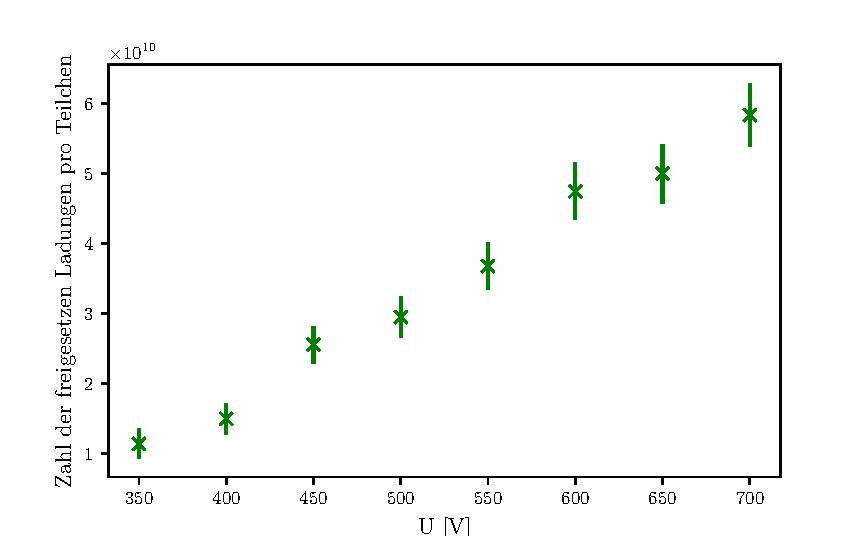
\includegraphics{plot1.pdf}
  \caption{Temperaturverläufe  der Reservoirs}
  \label{fig:temp}
\end{figure}

\subsection{b) Bestimmung der Näherungsfunktion}
Die Temperaturverläufe lassen sich am ehesten durch die Funktion $T(t)=At²+Bt+C$ 
beschreiben. Eine nicht-lineare Ausgleichsrechnung mit Python liefert folgende Koeffizienten:\newline
Temperaturreservoir 1:
\begin{align*}
& A = (-3.2249\cdot 10^{-4} \pm 4.1934\cdot 10^{-8})\ K/s²\\
& B = (0.0203 \pm 9.1105 \cdot 10^{-5} )\ K/s\\
& C = (294.9701\pm 0.0413)\ K\\
\end{align*} 
Temperaturreservoir 2:
\begin{align*}
& A = (9.5504\cdot 10^{-7} \pm 2.6711 \cdot 10^{-7})\ K/s²\\
& B = (-0.0112\pm 5.8032 \cdot 10^{-4})\ K/s\\
& C = (295.8702\pm 0.2634)\ K
\end{align*} 
Die Kurven sind in folgenden Plot dargestellt:
\begin{figure}
  \centering
  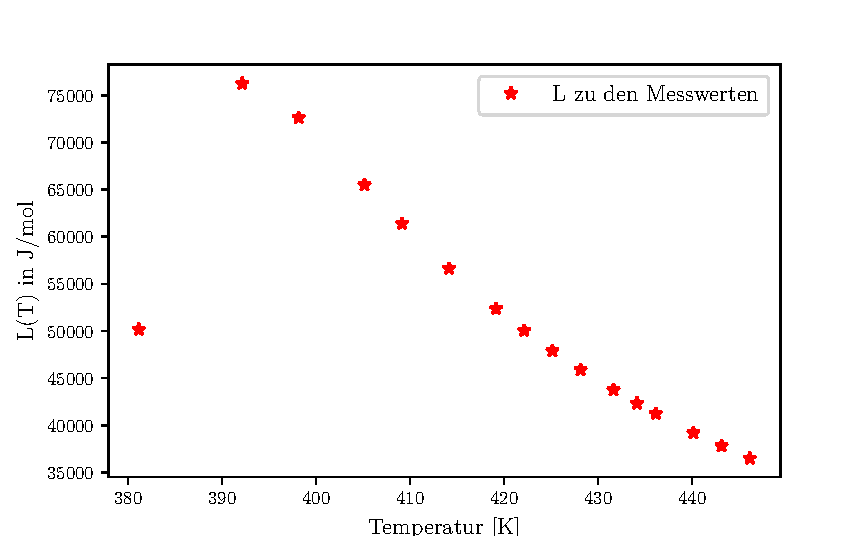
\includegraphics{plot2.pdf}
  \caption{Anpassung eines Polynoms 2. Grades}
  \label{fig:temp}
\end{figure}

\subsection{c) Bestimmung der Differentialquotienten}
Die Ableitung $\dfrac{dT}{dt}$ berechnet sich wie folgt:
\begin{align*}
  & \dfrac{dT}{dt}(t) = 2A \cdot t+B\\
\end{align*}
Für die Auswertung wähle ich folgende Wertepaare:
\begin{table}[H]
  \centering
  \caption{Ausgangswerte}
  \label{tab:data}
  \begin{tabular}{c c c c c}
    \toprule
    t[sec] & $T_1(t)$[K] & $T_2(t)$[K] & $\dfrac{dT_1}{dt}(t)$[K/s] & $\dfrac{dT_2}{dt}(t)$[K/s]\\
    \midrule
      300 & 300.7638 & 292.5935 & 0.0183 & -0.0106\\
      900 & 310.6097 & 286.5559 & 0.0145 & -0.0095\\
      1500 & 318.1338 & 281.206 & 0.0106 & -0.0083\\
      2100 & 323.3358 & 276.5436 & 0.0067 & -0.0072\\
    \bottomrule
  \end{tabular}
\end{table}




\subsection{d) Bestimmung der Güteziffer}
Die Güteziffer lässt sich durch $v = \dfrac{\Delta Q_1}{N\cdot \Delta t}$ berechnen.
Die pro Zeiteinheit gewonnene Wärmemenge erhält man durch die Berechnung von 
\begin{equation}
  \dfrac{\Delta Q_1}{\Delta t}=(m_1\cdot c_w+m_k\cdot c_k)\dfrac{\Delta T_1}{\Delta t}.
\end{equation}
Daher ergibt sich die reale Güteziffer als 
\begin{equation*}
  v=(m_1\cdot c_w+m_k\cdot c_k)\dfrac{\Delta T_1}{N\cdot \Delta t}
\end{equation*}
Die Güteziffer einer idealen Wärmepumpe lautet hingegen:
\begin{align*}
  v_{id}=\dfrac{T_1}{T_1-T_2}
\end{align*}
Folgende Größen sind gegeben:
\begin{align*}
  &m_1=4\ kg\\
  &c_w= 4.184\ J/kg\ K\\
  &m_k \cdot c_k = 750\ J/K\\
  &N=120\ W \text{  bzw.  } N=122\ W\\
\end{align*}
Somit erhält man für die Temperaturen aus c) die realen und idealen Güteziffern \\
\begin{table}[H]
  \centering
  \caption{Güteziffern}
  \label{tab:data1}
  \begin{tabular}{c c c c}
    \toprule
    $T_1(t)$[K] & $v_{real}$ & $\Delta v_real$ & $v_{id}$\\
    \midrule
      300.7638 & 2.6732 & 0.014 & 40.6284\\
      310.6097 & 2.1092 & 0.017 & 12.6321\\
      318.1338 & 1.5453 & 0.023 & 8.6899\\
      323.3358 & 0.9814 & 0.029 & 6.8238\\
    \bottomrule
  \end{tabular}
\end{table}
Die Güteziffern für $T_2$ sind im Idealfall gleich denen für $T_1$ und werden daher nicht erneut betrachtet.
Die realen Güteziffern liegen deutlich unter den idealen Güteziffern. Die idealen Güteziffern nehmen mit zunehmender
Temperatur allerdings auch sehr viel schneller ab als die realen Güteziffern.




\subsection{e) Berechnung des Massendurchsatzes}
Zunächst wird anhand von
\begin{equation}
  \label{eq: dadamm}
  \dfrac{\Delta Q_2}{\Delta t}=(m_2\cdot c_w + m_k\cdot c_k)\dfrac{\Delta T_2}{\Delta t}
\end{equation}
die aus Reservoir 2 entnommene Wärmemenge pro Zeiteinheit bestimmt. 
Für die vier Temperaturen beträgt sie 
\begin{align*}
  \dfrac{\Delta Q_2}{\Delta t}(t=300)=-185.9757\ J/s\\
  \dfrac{\Delta Q_2}{\Delta t}(t=900)=-165.9359\ J/s\\
  \dfrac{\Delta Q_2}{\Delta t}(t=1500)=-145.8961\ J/s\\
  \dfrac{\Delta Q_2}{\Delta t}(t=2100)=-125.8563\ J/s\\
\end{align*}
Zur Berechnung von L wird die Formel 
\begin{equation}
  \label{eq:L}
  \ln{(\dfrac{p}{p_0})}=-\dfrac{L}{RT}\ \Leftrightarrow \ L=-\ln{(\dfrac{p}{p_0})}RT
\end{equation} 
verwendet. Der Umgebungsdruck auf Meereshöhe beträgt etwa
$p_0=1 bar$. Die allgemeine Gaskonstante lautet $R=8.31446261815324
{\displaystyle \textstyle {\frac {\mathrm {kg\,m^{2}} }{\mathrm {s^{2}\,mol\,K} }}} $. Somit lässt 
sich L mittels linearer Regression aus folgender Grafik berechnen:
\begin{figure}[H]
  \centering
  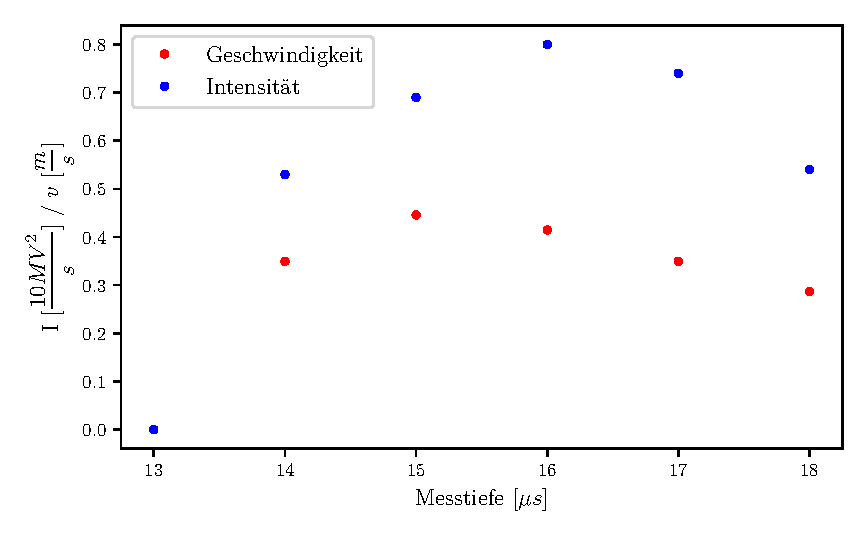
\includegraphics{plot3.pdf}
  \caption{Graph zur Bestimmung der Verdampfungswärme}
  \label{fig:L}
\end{figure}
Die Parameter der Ausgleichgeraden wurden bestimmt als:
\begin{align*}
  a=-2462.4863 \pm 70.5436\ K\\
  b=10.1354 \pm 0.2268
\end{align*}
Einsetzen in die Formel \eqref{eq:L} liefert:
\begin{equation*}
  L= - a \cdot R = 20474.2500 \pm 586.5324 \dfrac{J}{mol}
\end{equation*}
Mit der Formel \eqref{eq:neun} ergeben sich die Werte für den Massendurchsatz als 
\begin{table}[H] 
  \centering
  \caption{Massendurchsatz}
  \label{tab:data2}
  \begin{tabular}{c c c c}
    \toprule
    $T_1(t)$[K] & $\dfrac{\Delta m}{\Delta t}[mol/s]$ & $\dfrac{\Delta m}{\Delta t}[g/s]$ & Fehler\\
    \midrule
      300.7638 & -0.0091 & -1.0982 & 0.0697\\
      310.6097 & -0.0081 & -0.9798 & 0.0827\\
      318.1338 & -0.0071 & -0.8615 & 0.1051\\
      323.3358 & -0.0061 & -0.7432 & 0.1321\\
    \bottomrule
  \end{tabular}
\end{table}
Für die weiteren Berechnungen wurde mit der molaren Masse multipliziert. Diese erhält man durch Addition der
molaren Massen der einzelnen Stoffe des Gases zu 120.9 $\dfrac{g}{mol}$. \cite{wiki}


\subsection{f) mechanische Leistung des Kompressors}
Zunächst wird anhand der idealen Gasgleichung die Dichte \rho näherungsweise bestimmt.
\begin{equation}
  p=\rho \cdot R_s \cdot T
\end{equation}
Da $R_s$ konstant ist, folgt:
\begin{equation}
  \dfrac{p_0}{\rho_0 T_0}=\dfrac{p_2}{\rho T_2}
  \Leftrightarrow \rho=\dfrac{p_2 T_0 \rho_0}{p_0 T_2}
\end{equation}
Für die mechanische Kompressorleistung kann man dann, wie in der Theorie hergeleitet die Formel
\begin{equation}
  N_{mech}=\dfrac{1}{\kappa -1}(p_b \sqrt[\kappa]{\dfrac{p_a}{p_b}}-p_a)\dfrac{1}{\rho}\dfrac{dm}{dt}\\
  =\dfrac{1}{\kappa -1}(p_b \sqrt[\kappa]{\dfrac{p_a}{p_b}}-p_a)\dfrac{p_0 T_2}{p_2 T_0 \rho_0}\dfrac{dm}{dt}
\end{equation}
verwenden. Durch Einsetzen der Werte ergibt sich:
\begin{table}[H] 
  \centering
  \caption{Mechanische Kompressorleistung}
  \label{tab:data3}
  \begin{tabular}{c c}
    \toprule
    $T_1(t)$[K] & $N_{mech}[W]$ & Fehler \\
    \midrule
      300.7638 & $ 0.0897 $ & $ 0.0057 $ \\
      310.6097 & $ 0.1585 $ & $ 0.0134 $ \\
      318.1338 & $ 0.1785 $ & $ 0.0218 $ \\
      323.3359 & $ 0.1716 $ & $ 0.0305 $ \\
    \bottomrule
  \end{tabular}
\end{table}